\documentclass[12pt]{article}

\usepackage{array}
\usepackage{geometry}
\usepackage{graphicx}
\usepackage{changepage}
\usepackage{indentfirst}
\usepackage{CJKutf8}
\usepackage{color}
\usepackage{datetime}
\usepackage{indentfirst}
\usepackage{amssymb}
\usepackage{amsmath}
\usepackage{booktabs}
\usepackage{float}
\usepackage{lmodern}
\usepackage[T1]{fontenc}
\usepackage{textcomp}
\usepackage{cases}
\usepackage{bm}

\geometry{a4paper,scale=0.8}
\setlength{\parindent}{2em}

\renewcommand{\baselinestretch}{1.5}
\renewcommand{\today}{\number\year~年~\number\month~月~\number\day~日}

\title{计算机系统结构 lab2\\ \large{Tomasulo Simulator - report}}
\author{梅瑞虎 - 2016011335 - 计64}
\date{\normalsize\today}

\begin{document}

\begin{CJK}{UTF8}{gbsn}

\maketitle

\section{Tomasulo 总体框架}

本项目包含以下主要内容 (包含一个外部库, 但不涉及核心算法):

\begin{verbatim}
    code
    |----include
    |    |----tabulate/              # 表格输出外部库 (C++20)
    |    |----Inst.hpp               # 指令
    |    |----Reg.hpp      	         # 寄存器
    |    |----Station.hpp            # 保留站
    |    |----Unit.hpp               # 计算单元
    |    |----Tomasulo.h             # 算法模拟
    |    \----Util.h                 # 辅助函数
    |----src                         # 类方法实现
    |    |----Inst.cpp
    |    |----Reg.cpp
    |    |----Station.cpp
    |    |----Unit.cpp
    |    |----Tomasulo.cpp
    |    |----Simulator.cpp          # 函数入口
    |    \----Util.cpp
    \----CMakeList.txt               # cmake 配置文件
\end{verbatim}

\section{编译运行}

需要支持 \verb|C++20| 的 \verb|g++ make| 以及 \verb|3.10| 以上版本的 \verb|cmake|. 如下可正常编译运行:

\begin{verbatim}
    $ mkdir build
    $ cd build && cmake .. && make && cd ..
    $ ./bin/Tomasulo
\end{verbatim}

默认进行所有测试 (不包含自测样例), 输出到 \verb|log| 文件夹, 逐行对应测试文件指令. 对于因跳转指令未执行到的指令输出 \verb|`0 0 0'|.

\begin{verbatim}
    $ ./bin/Tomasulo [nel-path] [log-path]
\end{verbatim}

可通过以上命令进行单文件测试. 实验要求可查询任意 \verb|cycle| 的状态, 因此添加了单步执行输出, 见下列命令, 实现较简单, \verb|<flag>| 为任意字符(串)即可, 单步输出当前所有状态.

\begin{verbatim}
    $ ./bin/Tomasulo [nel-path] [log-path] <flag>
\end{verbatim}

\section{实现细节}

实验过程中, 先完成 \verb|NEL| 指令的读取分析, 再完成指令, 计算单元, 寄存器, 保留站等的实现. 最后实现了算法流程, 并在这一实现过程中, 对之前的模拟类进行了适当修改, 最终添加了输出和单步执行输出功能.

观察给出的样例测试, 指令执行完毕后, 受 \verb|RAW| 影响暂停的即可开始执行. 由这一现象, 得知整个流程图如下图.

由于未实现分支预测, \verb|Tomasulo| 整个流程的特性如下:

\begin{enumerate}
	\item 顺序发射. 发射指令均按指令顺序发射 (\verb|JUMP| 指令特殊).
	\item 乱序执行. 运行可执行指令条件为: 执行单元已分配, 操作数就绪. 与指令顺序无关.
	\item 操作数未就绪, 直接关联到保留站 (消除 \verb|WAR|).
	\item 指令一旦执行直至结束, 结束后无需条件即可写回, 同时更新依赖关系 (消除 \verb|WAW|).
	\item 发射停止条件为: 无指令可发射 (运行即将完毕), 或 \verb|JUMP| 指令发射且未执行完毕.
\end{enumerate}

\begin{figure}[H]
	\centering
	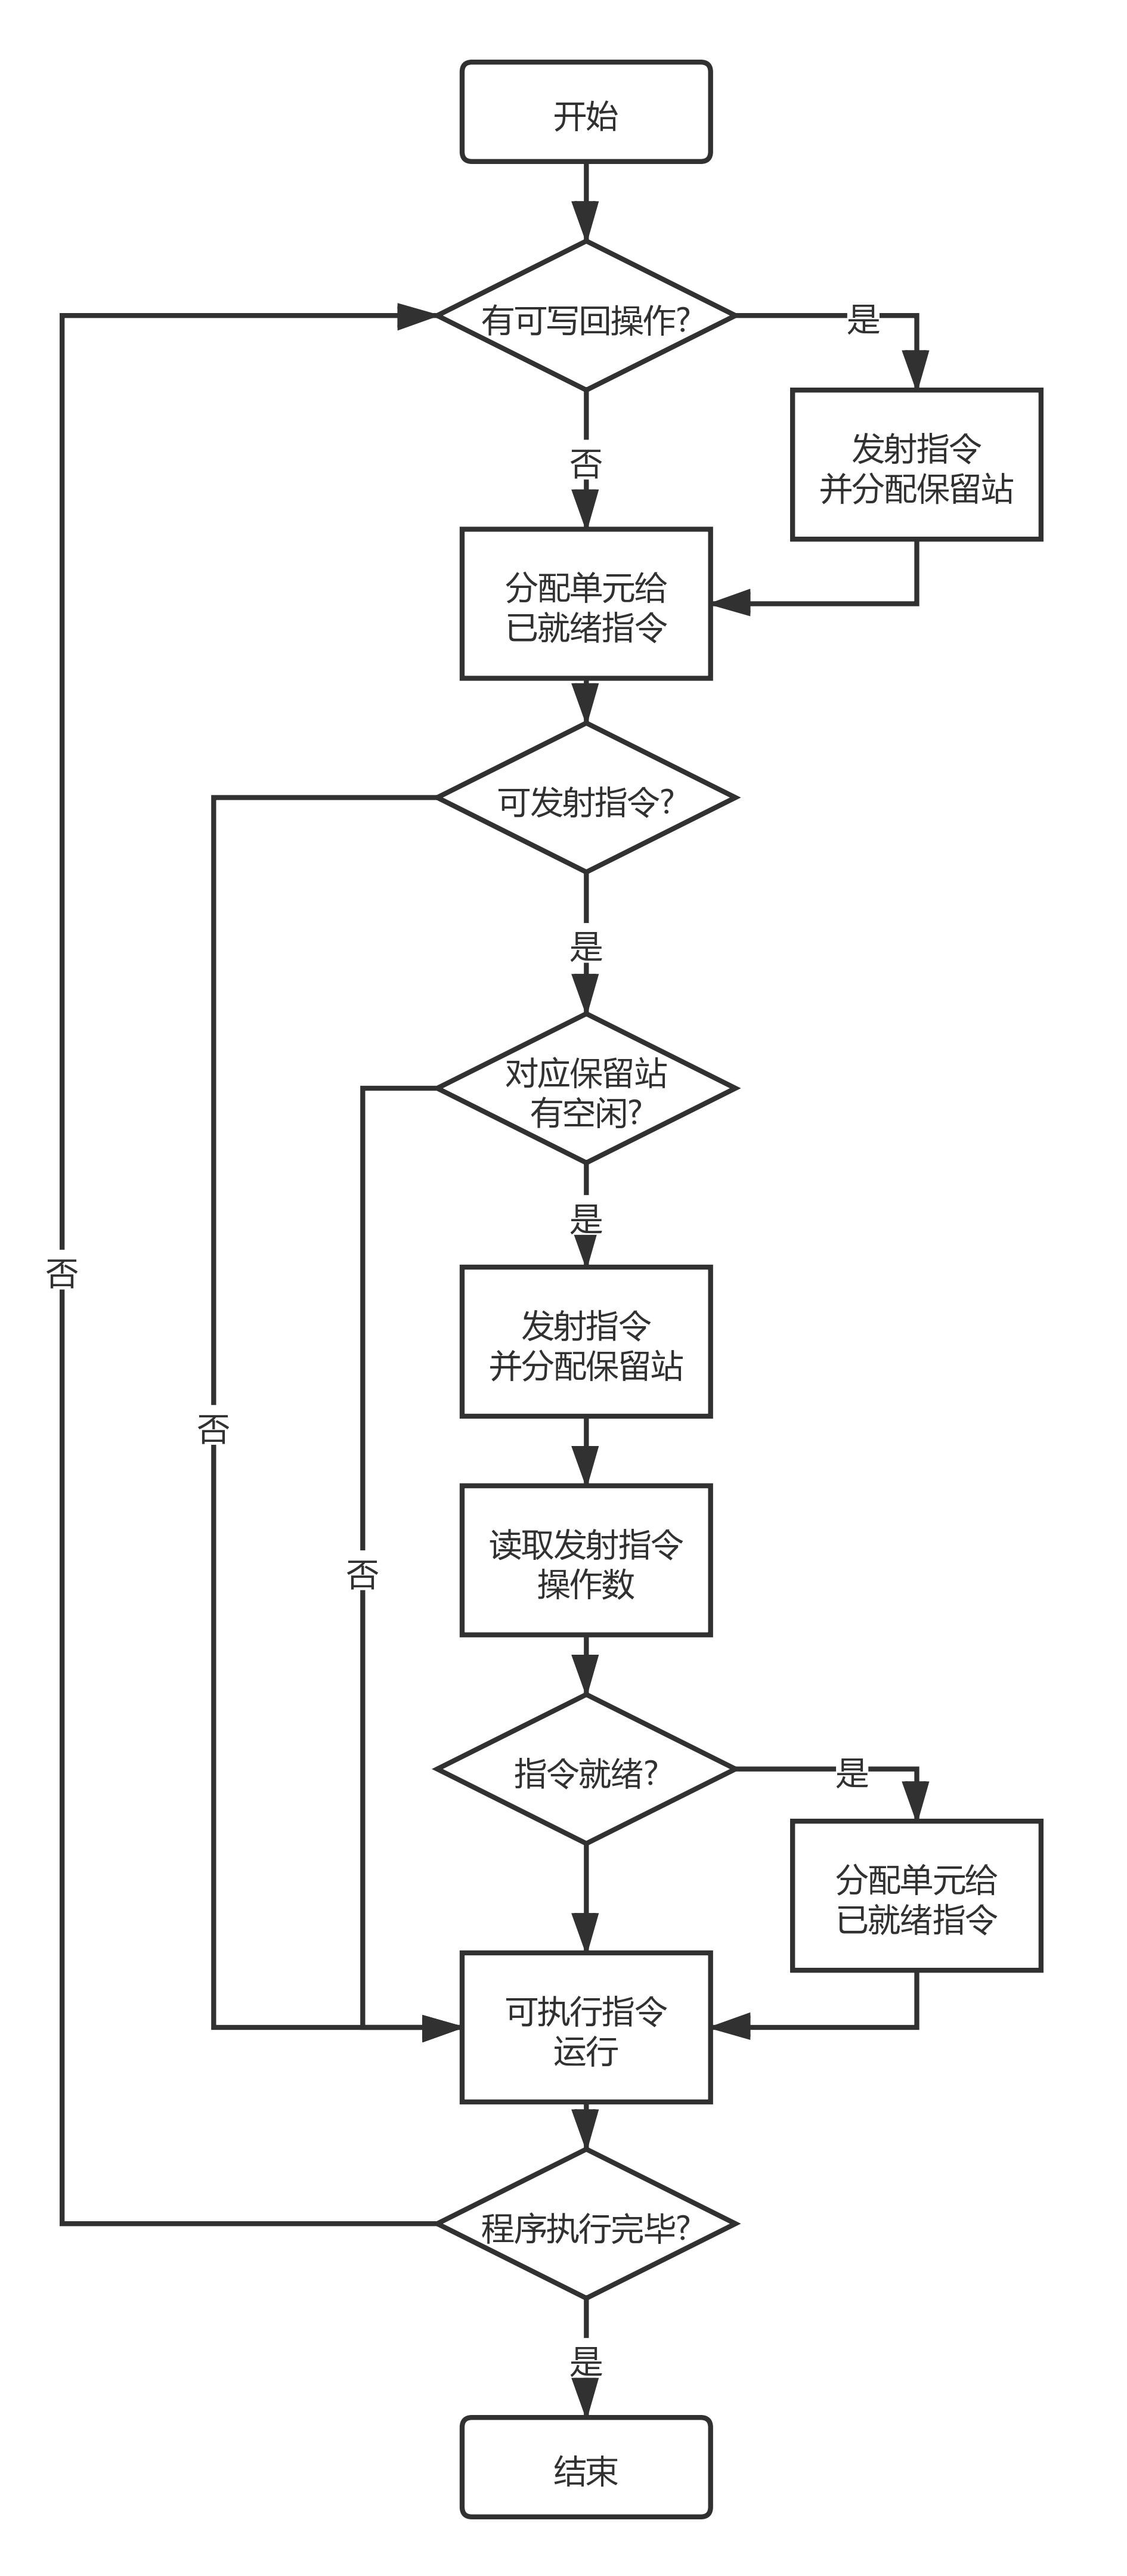
\includegraphics[width=0.5\linewidth]{img/flow}
\end{figure}

注意上图中的 \textbf{可执行} 和 \textbf{已就绪} 不同, 就绪指令在 \textbf{下一周期} 转变为可执行指令.

由 \verb|Tomasulo| 特性可知, 相比较记分牌算法, 其消除了 \verb|WAR| 和 \verb|WAW| 假相关. 究其根本类似编译原理专题训练中重点讲授的 ``Dataflow'', 即数据流算法框架.

对于 \verb|JUMP| 指令的实现, 简单实现了 \verb|PC| 寄存器. 在发射指令时, 根据 \verb|PC| 来发射, 在执行完 \verb|JUMP| 指令且需要跳转时, 对 \verb|PC| 进行修改. (实现中 \verb|PC| 为 \verb|nextIssueIndex|)

\section{实现结果}

进行了 \verb|Jump| 指令的实现, 未单独进行性能优化, 给出未优化下在测试机的运行时间:

\begin{verbatim}
    Big_test.nel  ->   2.73s
         Mul.nel  ->   0.01s
         Gcd.nel  ->  52.53s
\end{verbatim}

可见, 在课程给出的性能测试样例上, 模拟的效果比较好.

在 \verb|Gcd.nel| 样例上, 由于跳转次数极多导致运行时间较长.

\section{实验感想}

本次实验比较简单 (可能还有 bug), 仅额外实现了 \verb|JUMP| 并对此添加了简单测例 \verb|Jump.nel|, 用于测试存在指令未发射执行情况.

以上. 感谢老师的悉心指导和实验过程中助教的耐心解答!

\newpage

\end{CJK}

\end{document}